Die paarweise Kollisionserkennung bezieht sich auf die Kollision von zwei 3D-Modellen. In diesem Schritt ist die Genauigkeit der Kollision bei steigender Modellkomplexität im Fokus.
Ziel ist es die Diskrepanzen zwischen der grafischen Anzeige von Modellen und der physikalischen Simulation zu deckeln.
\subsection{Input}
Aus dem vorhergehenden Schritt der Kollisionspaarermittlung werden für den Schritt der paarweisen Kollisionserkennung bis zu  $|OBJ|^2$ Objektpaare $K_{guess}\subseteq OBJ^2$ erhalten, für die eine Kollisionsvermutung während eines Ticks gilt. Man geht weiter davon aus, dass die Menge der tatsächlichen Kollisionen $K_{definitive}\subseteq OBJ^2$ in der Menge der vermuteten Kollisionspaare  vollständig enthalten ist $K_{definitive}\subseteq K_{guess}$, d.h. keine tatsächlichen Kollisionspaare im Paarermittlungsprozess verlorengehen. Es ist eine Aufgabe dieses Schritts, die Reduzierung von $K_{guess}$ auf $K_{defintive}$ zu vollenden.

\subsection{Output}
Im Abschnitt~\ref{sec:usages} werden einige Verwendungszwecke der Kollisionsermittlung aufgelistet. 
Elemente der Aufzählung haben unterschiedliche Anforderungen hinsichtlich benötigter Information über den Kollisionsvorgang um realisiert werden zu können.

\begin{enumerate}
	\item Inklusion\\
		Die Frage ob Objekte $O_0, O_1 \in OBJ$ sich an einem konkreten Zeitpunkt während eines Ticks $t\in \Upsilon_{\delta i}$ schneiden/gegenseitig enthalten. $D(O_0, t) \cap D(O_1, t) \neq \emptyset$.
	\item Intrusion\\
		Die Frage nach den Eigenschaften
		\begin{enumerate}
		\item ob
		\item wann
		\item an welcher Raumposition
		\item mit welchen Teilen des Objektes
		\end{enumerate}
		ein Eindringen eines Objektes in ein anderes stattfindet, d.h. ein Zustandsübergang von Nicht-Kollision zu Kollision stattfindet.
		Hier beziehen wir uns auf die Zeitspanne eines Ticks $\delta_i$, während dem bei Zeitpunkt $\mathcal{T}(s)$ die erste Kollision (während $\delta_i$) auftritt. 
		$$\exists s \in [1, |\Upsilon_{\delta i}|-1], t_c= \Upsilon_{\delta i}(s):$$
		$$ D(O_0, t_c)\cap D(O_1, t_c) \neq \emptyset \wedge \forall s' < s: 
		D(O_0, \Upsilon_{\delta i}(s'))\cap D(O_1, \Upsilon_{\delta i}(s')) = \emptyset$$
		Aus der Schnittmenge $D(O_0, t_c)\cap D(O_1, t_c)$ können dann die Angeforderten Eigenschaften zur Kollision (Zeit, Ort, Beteiligte Objektteile) ermittelt werden.
\end{enumerate}
Es mag weitere Forderungen an Kollisionsalgorithmen geben. Die obige Aufzählung stellt dabei die von uns in Betracht gezogenen dar.

Für physikalische Verwendungszwecke insbesondere bei der rigiden Objektkollision scheint der Bereich der Intrusion mehr relevant. In Simulationen mit rigiden Kollisionsobjekten ist typischerweise der Zustand des Überschneidens zweier Objekte (Inklusion) nicht erlaubt und muss daher aktiv durch eine Kollisionsreaktion verhindert werden. Durch die Ermittlung des ersten Zeitpunkts des Bruchs der Nicht-Überschneidungsbedingung kann die Kollisionsreaktion passend ermittelt werden.\\
\begin{figure}
	\centering
	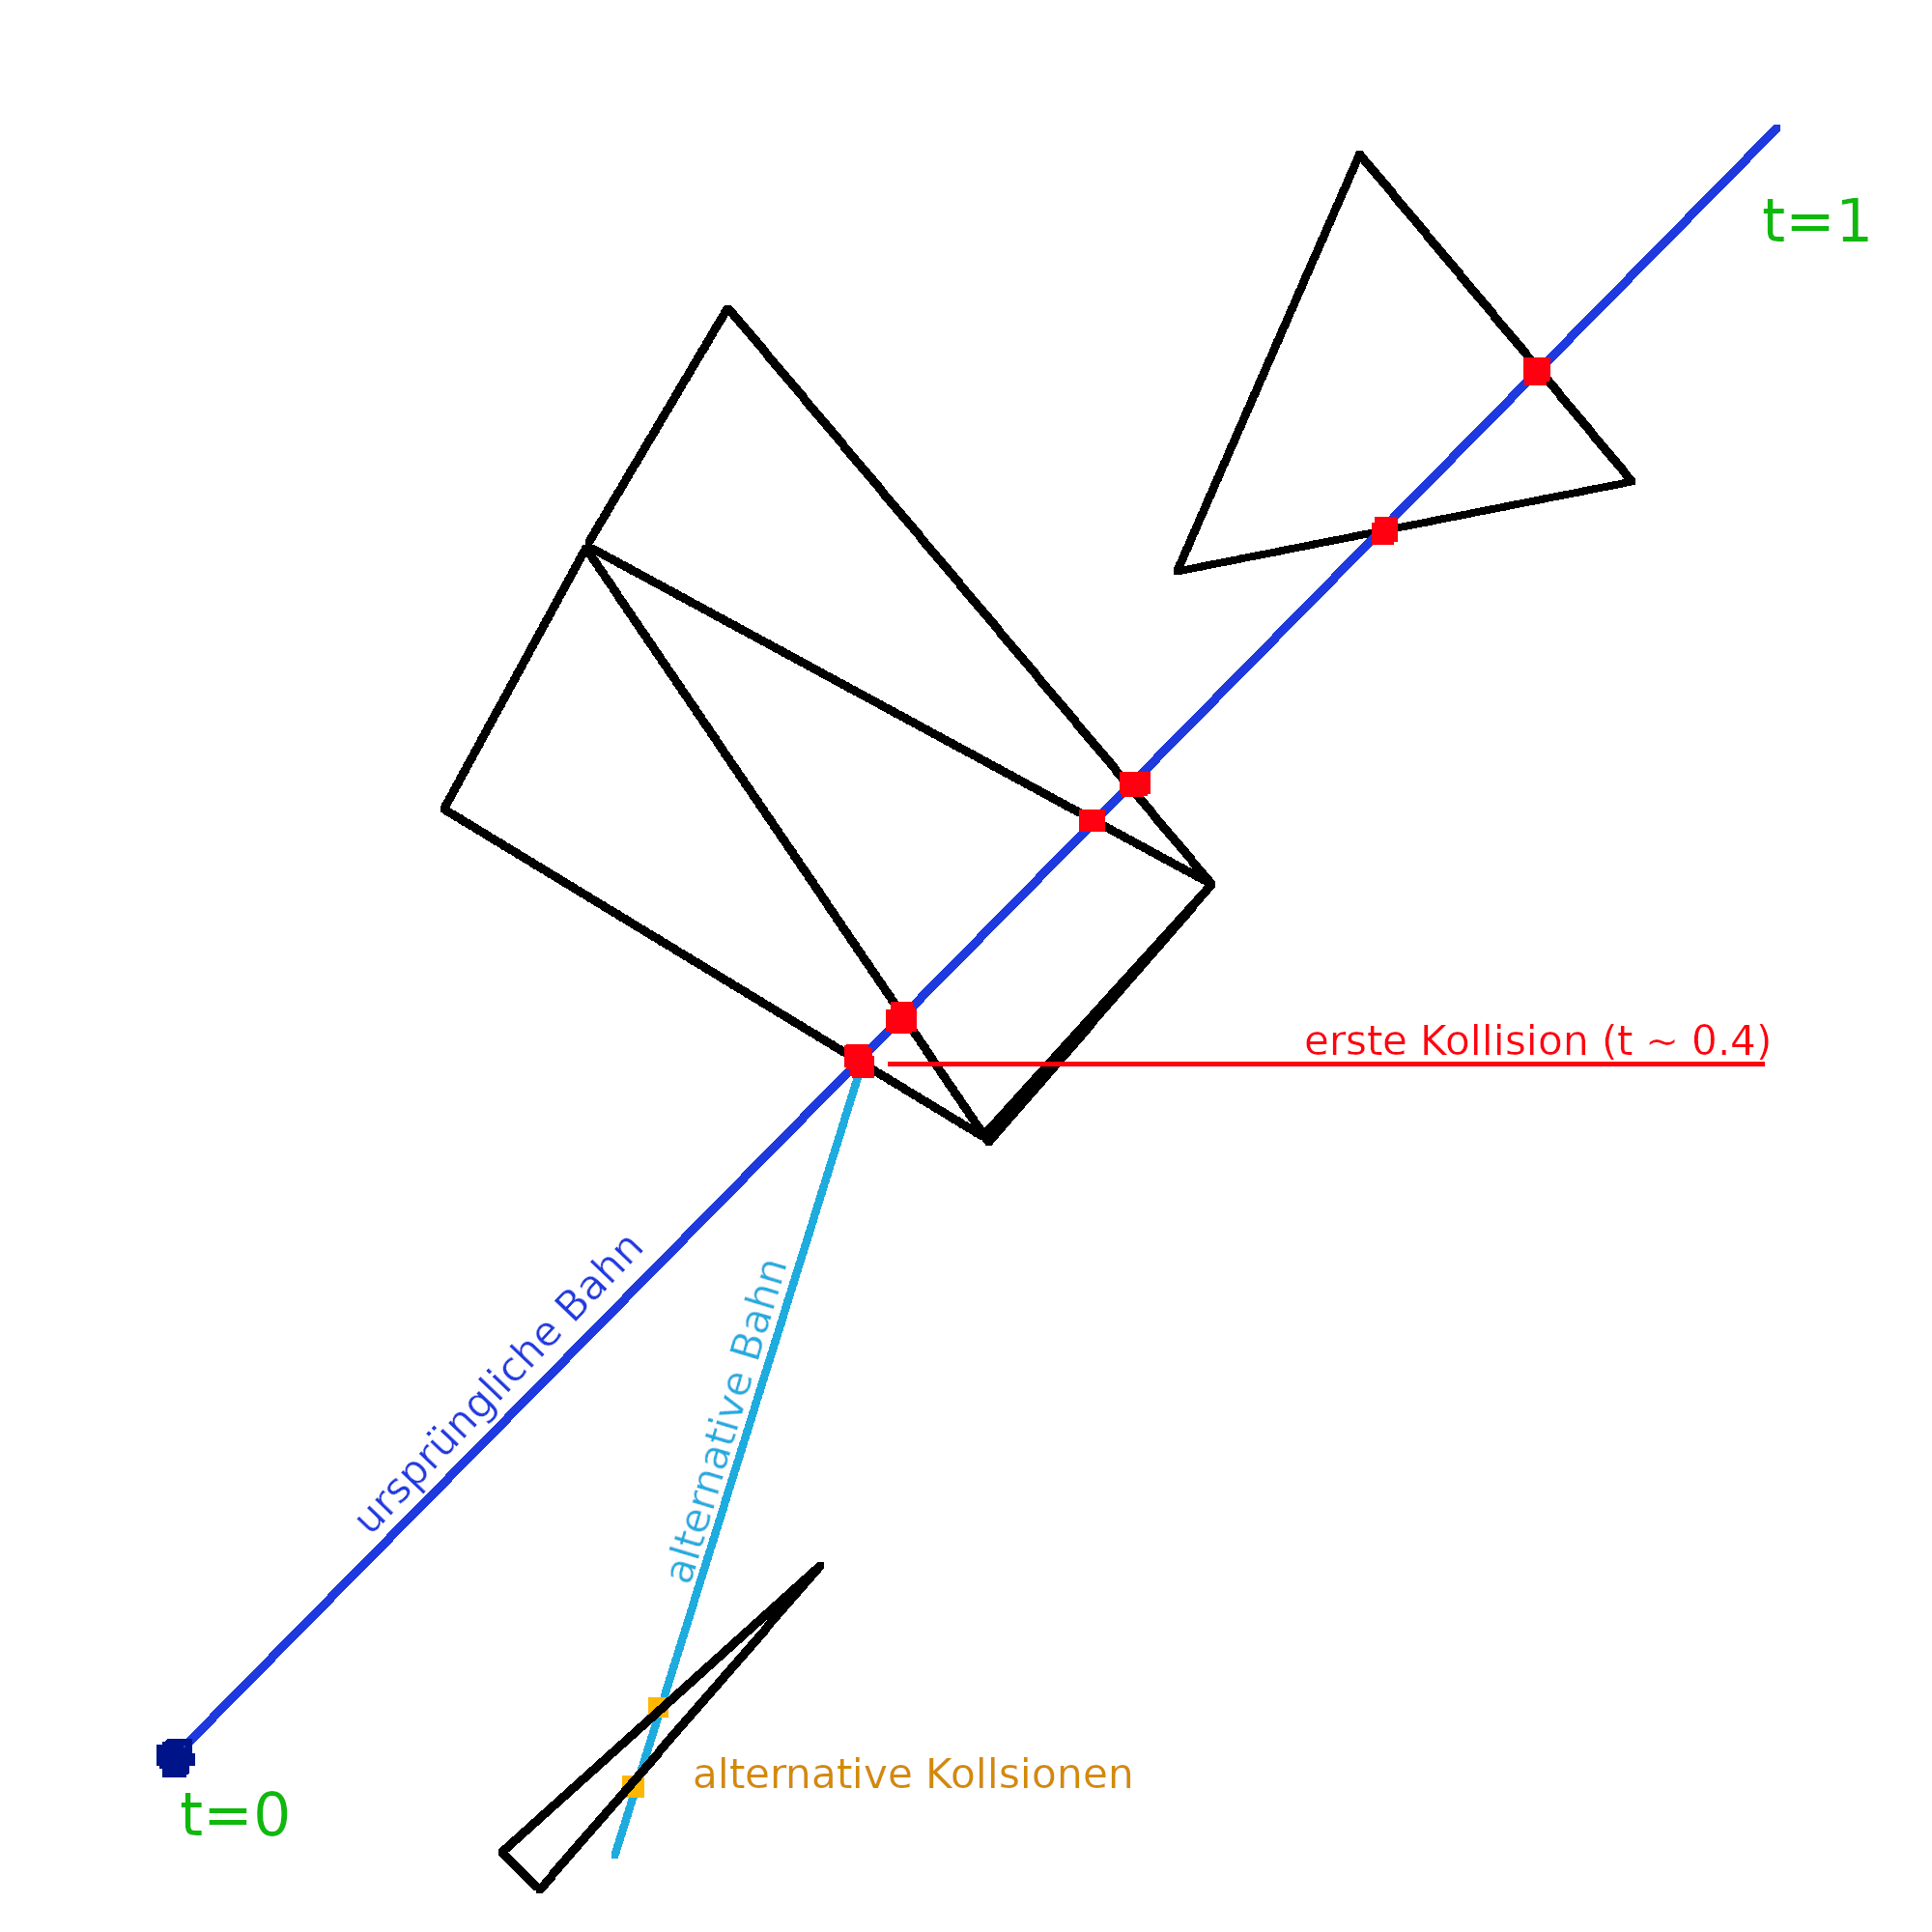
\includegraphics[width=0.6\textwidth]{./res/l3_col.png}
	\caption{2D Kollisionsszenario mit alternativen Bewegungsbahnen eines Projektils an Kollisionskörpern}
	\label{fig:l3col}
\end{figure}
Die Umsetzung der Auflösung von Kollisionen und Mehrfachkollisionen ist explizit aus diesem Projekt ausgeschlossen. Selbst jedoch bei der theoretischen Betrachtung von Mehrfachkollisionen während eines Ticks und Optionen zu deren Auflösung, bzw.~physikalischer Reaktion von Objekten , scheinen vorwiegend Erstkollisionen interessant zu sein. Man vergleiche hierzu Abbildung~\ref{fig:l3col}.\\
An dieser Stelle wird demnach die Annahme getroffen, dass zunächst nur Erstkollisionen durch Intrusion interessanter sind sind und zuerst ermittelbar gemacht werden sollten.


%%TODO look if one can fit that under his hat somewhere, would be rad 
%Ein interessanter Fehler bezogen auf L3 in freier Wildbahn ist in \cite{skyrimwallglitch} zu sehen. Es handelt sich dabei um einen Glitch im Spiel The Elder Scrolls V:Skyrim. Dabei wird eine gleichzeitige Kollision des Spielermodells (welches sich durch eine Ingame-Fähigkeit unüblich schnell bewegt), eines Objekts und einer Wand oder Tür provoziert. Die Kollision, bzw. die wiederholten Kollisionen zwischen dem Spielermodell, dem Objekt (Kessel/Teller/Korb) und der Wand/Tür werden nicht richtig aufgelöst, was dazu führt, dass der Spieler durch die Wand laufen kann.\\


\subsection{Intrusionsermittlung durch lineare Interpolation der Objektbewegung}
Um das Problem zu vereinfachen wird die zunächst die Rotation von Objekten vernachlässigt.\\
Genauer: In diesem Kontext erfährt ein Objekt $O\in OBJ$ während eines Ticks $\delta_i$ keine zeitliche Änderung der Rotation $\forall t \in \Upsilon_{\delta i} : rot(O, t) = rot(O, \Upsilon_{\delta i}(0))$. Dies hat mehrere Gründe:
\begin{enumerate}
\item Objekte hielten zum Start des Projekts noch keine Repräsentation für Rotation.
\item Rotation mit einzubeziehen wurde zu Anfang schon als schwierig eingestuft. Dieser Verhalt sollte sich später bestätigen.
\item Es gibt genügend Kollisionsszenarien/Verwendungszwecke für denen Rotation keine Rolle spielen muss. (Logische Kollision, Punktförmige Objekte, statische Objekte wie z.B. oft Terrain, Verwendungszwecke mit hoher Fehlertoleranz)
\item Es wird ein Experiment der Vernachlässigung von Rotation durchgeführt. Es soll dabei beantwortet werden, ob auch ohne Behandlung der Rotation eine ausreichend zufriedenstellende Illusion von physikalischem Realismus geschaffen werden kann.
\end{enumerate}

Wie in Abschnitt~\ref{sec:objects_mov} bereits beschrieben sind die zeitlichen Änderungen (Geschwindigkeit $v$ und Drehgeschwindigkeit $\omega$) eines Objektes während eines Ticks konstant. Durch die Vernachlässigung der Drehgeschwindigkeit $\omega$ kann die zeitliche Änderung eines Objektes $O$ allein auf Bezug zu Geschwindigkeit $v$ und der Zeit $t$ beschrieben werden, bzw.~alle im Objekt enthaltenen Punkte $p \in D(O, t_0)$ beschreiben lineare, parallele Flugbahnen.
$$l_p = \{p + (t - t_0) * v(O, t_0) | t_0 \leq t \leq t_1\}$$ 
Dies ermöglicht die Ermittlung von Kollisionen durch lineare Interpolation der Zeit.\\
Die Eigenschaft der Linearität hat dabei noch den weiteren entscheidenden Vorteil, dass bei einer Relativierung der Objekte wechselseitig zueinander, eine Operation der einer Transformation in Form einer Translation gleichkommt, die Linearität weiterhin gewahrt bleibt. Zum Vergleich: Mit aktiver Rotation beschrieben Objekte relativ zueinander Kurvenflugbahnen.\\
Es kann also wechselseitig zu beiden Objekten relativ gerechnet werden.\\
Wir definierten $D(O, t)$ als die Sammlung aller Flächen, Kanten und Ecken eines Objektes. Zur Vereinfachung benennen wir Objekte $O_x := (A_x, E_x, V_x)$ mit $A_x = A(O_x, t_0); E_x = (O_x, t_0); V_x = (O_x, t_0)$. Diese Merkmale sollen nun durch die Zeitdimension erweitert und dann kollidiert werden.
Es müssen nicht alle Merkmalskombinationen $\in \{Area, Edge, Vertex\}^2$ getestet werden. Es konnten essenzielle Merkmalskombinationen ermittelt werden, welche bei sich bei einer Erstkollision auftreten können:
		\begin{itemize}
			\item [$\{Vertex, Area\}$] Eine Ecke durchschlägt eine Fläche.\\
				$\Rightarrow$ Zu überpfüfende Paare: $(V_0\times A_1)\times (V_1\times A_0)$
			\item [$\{Edge, Edge\}$] Kanten durchschneiden sich gegenseitig.
				$\Rightarrow$ Zu überprüfende Paare: $(E_0\times E_1)\times (E_1\times E_0) = (E_0\times E_1)$
		\end{itemize}
		Alle anderen Kombinationen sind entweder in diesen beiden enthalten (z.B. $\{Vertex, Edge\}$ in 1.) oder eine Ereignis dieser beiden Szenarien muss logisch vorher passieren (z.B. 1. oder 2. muss vor $\{Edge, Area\}$ bereits passiert sein).
\ \\
		Aufgrund der Relativierung muss nur eines der Merkmale muss eine zeitliche Bewegung durchführen
		\begin{itemize}
			\item [$$\{Vertex, Area\}$$] 2 Möglichkeiten:
				\begin{itemize}
					\item[Option0:] Linie(Eckpunkt \& Zeitdimension) schneidet ein Dreieck\\
					Eckpunkt $v \Rightarrow l_v$
					\item[Option1:] Punkt schneidet ein schiefes Prisma(Dreicksfläche \& Zeitdimension)\\
					Dreiecksfläche $a \Rightarrow {l_p | p \in A_p(a)}$
				\end{itemize}
				Gewählt wird Option0, da einfachere Berechnung.
			\item [$\{Edge, Edge\}$]  Parallelogramm(Linie \& Zeitdimension) schneidet Linie
		\end{itemize}
\ \\
		Geometrische Eigenschaften nun beteiligter Formen:
		\begin{itemize}
			\item [Linie] $L = \{l | x\in\mathbb{F} ; l_0, l_1 \in \mathbb{F}^3 ; l = l_0 + x * l_1; 0\le x\le 1 \}$ \\
			mit Startpunkt $l_0$ und Endpunkt $l_0 + l_1$
		\item [Dreieck] $T = \{t | x,y \in\mathbb{F}; t_0, t_1, t_2 \in \mathbb{F}; t = t_0 + x*t_1 + y*t_2; 0\le (x+y) \le 1\}$\\
			mit Eckpunkten $a = t_0 ; b = t_0 + t_1 ; c = t_0 + t_2$ 
			\item [Parallelogramm] $P = \{p | x,y \in\mathbb{F}; p_0, p_1, p_2 \in \mathbb{F}; p = p_0 + x*p_1 + y*p_2; 0\le x\le 1; 0\le y\le 1\}$\\
			mit Eckpunkten $a = p_0 ; b = p_0 + 1.0*p_1 ; c = p_0 + 1.0*p_2; d = p_0 + 1.0*p_1 + 1.0*p_2$ 
		\end{itemize}
\ \\
		Beide Szenarien können über Gleichungssysteme zur Ermittlung der Koeffizienten in konstanter Zeit überprüft werden:
		\begin{itemize}
			\item [$\{Vertex, Area\}$] $l_0 + x * l_1 = t_0 + y*t_1 + z*t_2$\\
				$x$ ist zudem hier der Koeffizient der Zeit, da die Linie in der Zeitdimension liegt.
			\item [$\{Edge, Edge\}$] $l_0 + x * l_1 = p = p_0 + y*p_1 + z*p_2$\\
				Sei die ursprüngliche Linie, aus dem das Parallelogram generiert wurde $p_0+y*p_1$, so liegt die andere Linie $p_0 + z*p_2$ in der Zeitdimension und somit ist hier z der Zeitkoeffizient.
		\end{itemize}
\ \\
		Komplexität:
\begin{itemize}
			\item [$\{Vertex, Area\}$] $|V(O_0, t_0)|* |A(O_1, t_0)| + |V(O_1, t_0)|*|A(O_0, t_0)|$
			\item [$\{Edge, Edge\}$] $|E(O_0, t_0)| * |E(O_1, t_0)|$
		\end{itemize}
\ \\
		Eigenschaften der Kollisionserkennung von linearer Interpolation unter den getroffenen Annahmen:
		\begin{itemize}
			\item mathematisch exakte Ermittlung der Zeit einer Kollision
			\item mathematisch exakte Ermittlung des Orts einer Kollision
			\item Ermittlung der Beteiligen Objektmerkmale
			\item Zuverlässige Ermittlung der ersten Kollision (durch zeitliche Sortierung der einzelnen Merkmalskollisionen)
		\end{itemize}
Probleme:\\
Der Einsatz der linearen Interpolation ist im Kontext eines Videospiels recht beschränkt.
Es scheint nicht möglich sie effektiv auf die beschriebene Art und Weise einzusetzen um Kollisionen bei rotierenden Körpern zu erkennen.
Für lineare Interpolation wird ein Fazit gezogen:
\begin{itemize}
	\item Ohne Rotation ist der Ansatz exakt und erfüllt alle gestellten Anforderungen.
	\item Praktisch immernoch in vielen Fällen gut einsetzbar. Beispiel: Punktförmiges Projektil gegen unbewegliches Terrain.
\end{itemize}

\subsubsection{Gilbert-Johnson-Keerhi-Algorithmus (GJK)}
GJK ist ein Algorithmus zur Berechnung der minimalen Distanz zwischen konvexen Sets, publiziert 1988 \cite{gjk}, der in vielen Kollisionverfahren eingesetzt wird.\\
		Der Algorithmus wird in vielen Videospielen verwendet, beispielsweise in Blizzard Entertainments Diabolo 3 (\cite{gdc-physics}) und Valves Half-Life 2(\cite{gjk-blog}).\\
		
		Seien die Objekte $K_0, K_1$ als kompakte Mengen von Raumpositionen gegeben, welche ein Objekt einnimmt.\\
		Die Menge $M = \{c | c = a - b; a\in K_0 ; b\in K_1\}$ denotiert dabei die so genannte Minkowski-Differenz, deren Eigenschaften in diesem Verfahren ausgenutzt werden.\\
		\begin{enumerate}
			\item Die Minkowski-Differenz zweier konvexer Körper ist ebenfalls konvex.
			\item Kollidieren/Überschneiden sich die Objekte $K_0, K_1$ so ist die Menge $K_0 \cap K_1$ nicht leer und so gilt, dass der Ursprung $O := (0,0,0)$ in der Minkowski-Differenz enthalten ist, da $\exists a_o, b_o \in K_0 \cap K_1 : a_o = b_o \Rightarrow a_o - b_o = O \Rightarrow O \in M_{K_0, K_1}$.
			\item Der Ursprung markiert im Bezug auf $M$ die Distanz zwischen zwei Objekten, wobei die Distanz hier nicht die zwischen den einzelnen Objektursprüngen ist, sondern die minimale euklidische Distanz zwischen zwei Punkten der Objekte $distance: \mathbb{R}^3 \times \mathbb{R}^3 \mapsto \mathbb{R}; distance(K_0, K_1) = min\{|a - b| : a \in K_0 , b\in K_1\}$. Der näherste Punkt zum Urspung $P\in M$ hat die selbe Distanz wie die Objekte zueinander, wenn keine Schnittmenge besteht $if K_0 \cap K_1 = \emptyset \Rightarrow distance(P, O) = distance(K_0, K_1)$
			\item Für den Fall $O \in M$ kann durch den Abstand zur konvexen Hülle $\mathcal{H}(M)$ eine Penetrationsziefe ermittelt werden, welche allerdings richtungslos ist, d.h. minimale Penetrationstiefe, nicht Penetrationstiefe bei Penetration von einer bestimmten Richtung.
		\end{enumerate}
		Die Berechnung von unendlich großen Mengen von Punkten ist jedoch berechnungstechnisch nicht praktikabel. Als Objektrepräsentation werden hier, wie auch in anderen 3D-Anwendungen üblich, stattdessen Ecken und Kanten der Hülle eines Objektes angegeben. Die entstehende diskrete Minkowski-Differenz $M_d$ ist daher nicht mehr kompakt. Die Verwendung der relevanten Eigenschaften der Minkowski-Differenz weicht deshalb etwas von der theoretischen Mengensemantik ab.
Eine Illustation unter diesen Umständen ist in den Abbildungen \ref{fig:minkov_col}, \ref{fig:minkov_col_solo} und \ref{fig:minkov_noncol}zu sehen. Zu sehen sind, in Rot und Blau, die 2 Objekte, welche sich in \ref{fig:minkov_col} überschneiden und in \ref{fig:minkov_noncol} nicht. Die Gebilde, deren Ecken grün sind und deren Kanten rot und blau sind sind die jeweiligen Minkowski-Differenzen.
Die grünen Punkte sind alle Punkte, die durch die Anwendung der Minkowski-Different auf die Menge der Eckpunkte beider Körper ermittelbar sind.\\
Die Kanten sind rot oder blau, je nachdem von welchem Ursprungskörper eine Kante Einfluss erhält. So ist die Beteiligung beider Körper an der Differenz besser zu erkennen. Theoretisch sind auch die Kanten zwischen jedem Punktepaar mit gemischten Einflüssen der beiden Ursprungsobjekte darstellbar, welche aus Darstellungsgründen nicht in der Grafik enthalten sind. Isoliert steht in Abbildung \ref{fig:minkov_col_solo} die Minkowski-Differenz aus Abbildung \ref{fig:minkov_col}.\\
An dieser Stelle wird auch festgehalten, dass das erhaltene Gebilde kein Hüllenobjekt mehr ist, da nun auch Punkte und Kanten im Innenraum bekannt sind.\\
\\
Um die Überschneidung der Objekte festzustellen, wird ermittelt, ob $O\in M$.\\
$K_0, K_1$ sind konvex, daher ist $M$ ebenfalls konvex. Zwischen allen Punkten in einem konvexen Set existiert eine gerade Linie, die sie verbindet und die ebenfalls komplett im selben konvexen Set enthalten ist $\forall (P_0, P_1)\in M^2 : 0 \le x \le 1 ; (P_0 + P_1*x) \in M$. Dies gilt auch für $O$, wenn $O\in M \Rightarrow \exists (P_{O0}, P_{O1}) \in M^2 : P_{O0} + P_{O1}*x = O$.\\
Die Restriktion auf $M_d$ verhindert allerdings die Verwendung dieser Eigenschaft, da die benötigten Punkte $(P_{O0}, P_{O1})$ nicht zwingen in $M_d$ enthalten sind, um die Verbindung zum Ursprung direkt herzustellen.\\
Da der Ursprung also nicht direkt gesucht werden kann, wird versucht ihn einzugrenzen. Ist es möglich den Ursprung mit einem Simplex(im 3D-Fall ein Tetrahedron) mit Eckpunkten $v_i \in M_d$ zu umschließen, so ist $O\in M$.\\
Der Algorithmus lautet wie folgt:
\begin{itemize}
	\item[1.] Starte an beliebigem Punkt $P_0 \in M_d$
	\item[2.] Simplex $S = {P_0}$
	\item[3.] Setze Richtung $D = -P_0$
	\item[4.] Finde $P_{\#S}$, einen neuen Punkt für $S$, den maximalen Punkt in der Richtung $D$\\
		Da $M$ konvex, existiert dieses Maximum in jede Richtung. Ermittelt wird dieser Punkt über die Größe des Skalarproduktes $P_1 = max\{D \cdot P_i ; P_i \in M_d\}$
	\item[5.] Befindet sich der Ursprung noch hinter $P_{\#S}$ in Suchrichtung ist er nicht in $M$ enthalten, was ebenfalls über das Skalarprodukt ermittelbar ist $-P_{\#S} \cdot D > 0 \Rightarrow$ Frühzeitiger Abbruch, bzw. Ermittlung des nähersten Merkmals und dem Abstand zum Ursprung zur Distanzbestimmung.
	\item[6.] $S \cup {P_{\#S}}$ Ermittle das näheste bekannte Merkmal. Die Art des bekannten Simplex hängt von der Größe von $S$, $\#S$ ab.
		Gesucht wird immer das näherste Merkmal zum Ursprung. Darauf folgt Änderung der Suchrichtung in Richtung des Ursprungs orthogonal zu diesem Merkmal.
		Dabei wird $S$ mit den Punkten des Merkmals übeschrieben und $D$ mit der neuen Richtung.
		Wird bei $\#S$ festgestellt, dass sich der Ursprung im inneren des Tetrahedrons befindet, wurde die Kollision festgestellt.
		Beispiel:\\
			$\#S=2$: Linie $L_{P_0,P_1} = {P_O + x * P_1; 0\le x\le 1}$\\
				%TODO check theory
				Da von $P_0$ aus gesucht wurde und $P_1$ maximal $\Rightarrow$ $Linie L_{P_0,P_1}$ ist am nähersten am Ursprung.\\
				Setze $D$ in die Richtung des Ursprungs orthogonal zu der Linie zwischen $ P_0, P_1 $, welche berechnet werden kann durch $L_0 \times OP_1 \times L_0$.
	\item[7.] gehe zu 4.
\end{itemize}
Mit diesem Algorithmus können zwei statische 3D-Objekte auf Überschneidung überprüft werden. Der Algorithmus ist demnach eine Lösung für das Inklusionsproblem.\\

\begin{figure}
	\centering
	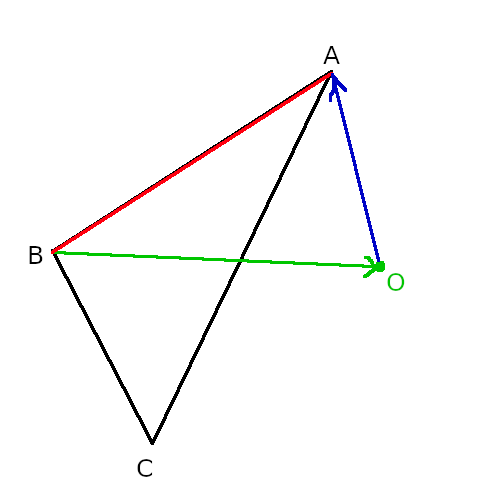
\includegraphics[width=0.6\textwidth]{./res/why_criteria.png}
	\caption{Szenario, in dem das gezeigte Abbruchskriterium nicht am nähesten Merkmal zum Ursprung stoppt.}
	\label{fig:why_criteria}
\end{figure}

Der bisher dargestellte Algorithmus löst jedoch nicht das Problem der Distanzfindung. Nachdem der Algorithmus in 5.~ abbricht, muss weiter nach dem nähesten Merkmal am Ursprung gesucht werden. Die Grafik \ref{fig:why_criteria} zeigt dabei, dass das bisherige Abbruchkriterium aus 5. nicht ausreicht.
Dort zu sehen ist das schwarze Dreieck $ABC$ und der grüne Ursprung $O$. Angenommen der Algorithmus beginnt an Punkt $B$ und sucht in Richtung des Ursprungs (grüner Pfeil) so wird als nächster Supportpunkt A gewählt und somit die rote Linie gefunden. Das Abbruchkriterium prüft nun, ob der Ursprung noch hinter diesem maximalen Punkt in der Suchrichtung läge, was durch das Skalarprodukt zwischen dem blauen und dem grünen Pfeil festgestellt wird (Schritt 5). In dem in der Grafik gezeigten Szenario führte dies zum Abbruch. Das gefundene Merkmal $AB$, die rote Linie, ist jedoch nicht das näherste am Ursprung. Das näheste Merkmal am Ursprung wäre stattdessen die Linie AC.\\
Prinzipiell ist das weitere Vorgehen des Algorithmus wie folgt zu beschreiben:\\
Suche neues Vertex in Richtung des Ursprungs bis keine weitere Annäherung mehr erfolgt.\\
Es wurden verschiedene Versuche unternommen das Kriterium einfach umzusetzen:
\begin{enumerate}
	\item Das Simplex, welches durch die bekannten Punkte aus $S$ gebildet wird besitzt eine minimale Distanz zum Ursprung, der errechnet werden kann. Verringert sich dieser Abstand nicht durch Erweiterung um den neuen Support-Punkt $P_{\#S}$ in 4. wird abgebrochen. Die Lösung bedient sich dabei anderen mathematischen Routinen, wie z.B. Normalisierung (welche Division verwendet) und wird daher zwar als trivial, aber auch als relativ komplex angesehen.
	\item Neue Support Punkte sind nach 4.~ maximal. Ist das näherste Merkmal erreicht, so wird nach 4.~in eine Richtung gesucht, deren maximale Punkte bereits bekannt sein müssen. Daher ist ein mögliches Abbruchkriterium: Abbruch beim finden eines Support-Punktes, der bereits bekannt ist. Dieses Kriterium kann in Konstantzeit abgeprüft werden, da die bekannten Supportpunkte eine maximale Anzahl von 3 Annehmen können.
	\item Ein neuer Support Punkt soll eine Erweiterung in die Suchrichtung darstellen. Seien $S$ die bekannten Support-Punkte und $P_{\#S}$ der neu gewonnene. Nehmen wir die Suchrichtung als Ebenennormale an, liegt das von den in $S$ enthaltenen Punkten gebildete Simplex in der dieser Ebene. Alle neuen Punkte, welche eine Erweiterung in Richtung des Ursprungs darstellen sollen, müssen in Richtung der Ebenennormale liegen. Dies ist festzustellen, in dem Vektoren $V := P_{\#S}-s_i ; s_i\in S$ auf ein positives Skalarprodukt mit der Suchrichtung überprüft werden. Abbruchkriterium: $\exists V : D \cdot V <= 0$. Idee: Wird ein koplanarer oder gar schon bekannte Support-Punkt gefunden ist das Skalarprodukt $0$ und der Abbruch wird eingeleitet, da keine Erweiterung mehr schaffbar ist.
\end{enumerate}
Bei der Implementierung der Abbruchkriterien wurden jedoch Probleme erkennbar. Bei Abbruchkriterien 2 und 3 konvergierte der Algorithmus regelmäßig nicht. Es wurden folgende Fehler gefunden:
\begin{enumerate}
	\item Falsche Annahme: Das näherste Merkmal der Markovsumme ist eindeutig.\\
	Generierbare Simplices in der Markovsumme können überlappen (z.B. aber nicht ausschließlich mit anteilig gleichen Eckpunkten bei Dreiecken). Es können demnach mehrere nächste Simplices zum Ursprung existieren.\\

\begin{figure}
	\centering
	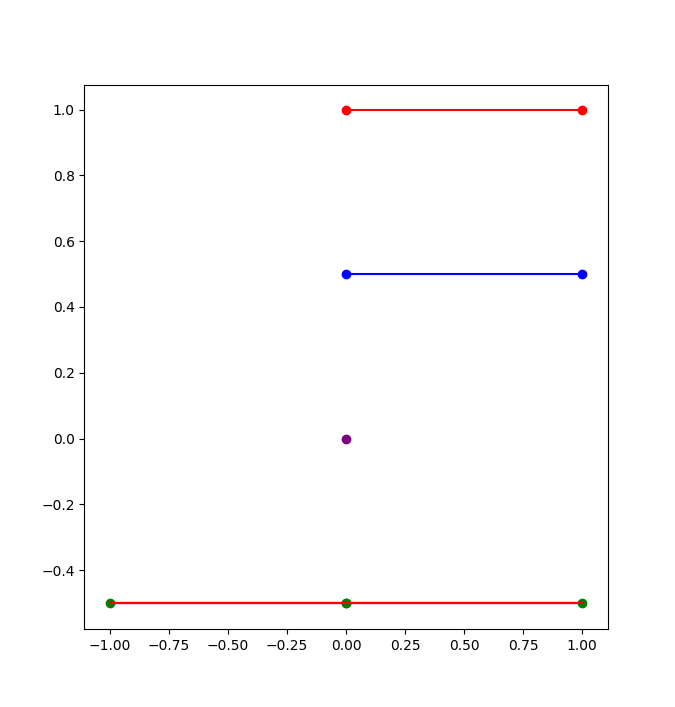
\includegraphics[width=0.6\textwidth]{./res/parallel_features.png}
	\caption{Szenario, in dem das gezeigte Abbruchskriterium nicht am nähesten Merkmal zum Ursprung stoppt.}
	\label{fig:parfeat}
\end{figure}

		Die Grafik \ref{fig:parfeat} zeigt ein solches Szenario. Oben im Bild, die rote und blaue Linie, geben die Ursprungsobjekte an. Der Ursprung ist in violett zu sehen. Die unten im Bild befindliche Linie ist die Markovsumme der roten und blauen Linie. An dieser zu sehen, in Grün, sind die generierten Eckpunkte. Die koplanarität erlaubt dem Algorithmus das Ignorieren des mittleren grünen Punktes. Demnach sind hier der mittlere Punkt und die Linie, welche die beiden äußeren Punkte verbindet exakt gleich weit vom Ursprung entfernt, genauso sind die Linien von jeweils einem Punkt von außen zur Mitte, und ein Dreieck aus allen grünen Punkten.

	\item Falsche Annahme: Verwendete Funktionen sind ausreichend genau.\\
		Theoretisch sollten (nahezu) koplanare Merkmale dieselbe neue Suchrichtung erzeugen. Daraufhin neu gefundene Support-Punkte sind deterministisch (Reihenfolge der Markovpunkte in der Maximumssuche ist immer gleich, Maximumssuche ebenfalls deterministisch). Ungenauigkeiten bei der Suchrichtungsermittlung arbeiten jedoch diesem Determinismus entgegen und erzeugte bei (unter floating Point präzision) nahezu gleichen Eingaben unterschiedliche Punkte, wenn eine auswahl von nahezu koplanaren Punkten existiert. Mehr noch: Alle neuen Punkte skalierten dabei regelmäßig auf Grund der Ungenauigkeit auch noch positiv mit der Suchrichtung was zur Folge hat das Abbruchkriterien 2 und 3 zu keiner konvergenz führten und den Worst Case einer Endlosschleife annehmen.\\
	Die Ungenauigkeit wurde auf die Kondition des Kreuzproduktes zurückgeführt, welches hauptsächlich zur Ermittlung der orthogonalen Suchrichtung verwendet wird. Das ursprüglich als zu komplex angesehene Abbruchkriterium 1 arbeitet nicht mit der aus Kreuzprodukten erzeugten Suchrichtung, sonder direkt auf den bekannten Merkmalen, verwendet selbst keine Kreuzprodukte und wird daher die einzig verbleibende Option. Das Kriterium führte auch in allen Tests erfolgreich zur Konvergenz.
\end{enumerate}
~\\
Weiter ist der Algorithmus bis jetzt nur ein statischer Intersektionstest. Um aus dem Inklusionsalgorithmus einen Intrusionsalgorithmus zu machen, wird eine Nullstellensuche auf die erhaltene Distanz angewandt.
Das Wurzelsuchverfahren hat zudem den Vorteil, dass es unabhängig von der Bewegungsart der Objekte ist. Animation, Rotation oder beliebige Transformation ist prinzipiell denkbar, solange über eine stetige Distanzfunktion abstrahiert wird.\\
Insbesondere im Falle der Rotation sind Überlegungen zu Startpunkten der Suche and der Distanzfunktionskurve anzustellen. Bei einer schnellen Rotation kollidieren Objekte unter Umständen mehrfach hintereinander, mit kollisionsfreien Episoden dazwischen. Bei Betrachtungen der Intrusion können Nullstellen sowohl beim Ein- als auch beim Austritt festgestellt werden.\\
Die Distanzfunktion verhält sich bei rotierenden Körpern wie eine Schwingung. Es gilt das Nyquist-Shannon-Abtasttheorem. Um beispielsweise die erste Nullstelle/Kollision zu finden ist die Rotationsgeschwindigkeit eines Objektes von Bedeutung, um den Suchraum bedeutend einzugrenzen.\\
Desweiteren ist an dieser Stelle festzustellen, dass das Verfahren wieder durch die Rotationsgeschwindigkeit beschränkt wird.
\\
Des weiteren bleibt ein Problem mit der Restriktion auf konvexe Objekte mit diesem Ansatz. 
Nicht-konvexte Objekte können in konvexe Objekte aufgetrennt werden. Praktisch wird diese Trennung meist extra mit dem Modell angegeben. Dabei sind in der Industrie die Form des tatsächlichen Modells und den zur Kollision angebenen Formen oft nicht kongruent und stellen daher inakkurate Hitboxen dar.\\
Automatisierte Methoden der Aufteilung sind komplex. Prinzipiell, für den Fall dass Objekte rigide sind, ist eine solche Aufteilung 1-mal Aufwand und daher Echtzeitfähig. Sind Objekte jedoch flexibel, z.B. durch Animation an Gelenken, müsste eine automatisierte Aufteilung bei jeder Änderung, u.U.~ mehrere male pro Tick auf ein Objekt angewendet werden. Das wäre Echtzeitfähig nicht tragbar. Deshalb werden in vielen Videospielen Gelenke ignoriert oder durch Kugeln approximiert.\\
Eine Familie nicht-konvexer Objekte, welche aus konvexen Objekten aufgebaut ist, ist prinzipiell noch abdeckbar. Dabei ist wiederholtes Verwenden des GJK-Algorithmus für jedes Teilobjektepaar verschiedener Ursprungsobjekte vonnöten. \\
Es lohnt sich, konvexe Teilobjektpaare durch andere Verfahren vorzufiltern und auszuschließen, wenn möglich.\\
Möglicher Ansatz hierfür ist z.B.~ wieder AABB-Pruning (wir bereits aus L1 bekannt).
\\
Überprüfung der erfüllung gestellter Anforderungen aus L3:\\
\begin{itemize}
	\item Die Kollision wird ermittelt
	\item Die Kollisionszeit wird in einem bestimmten Genauigkeitsrahmen während der Wurzelsuche bekannt.
	\item Die beteiligten Merkmale können aus den ermittelten nähersten Supportpunkten zurückgerechnet werden. Dazu werden zu den Supportpunkten die Quellpunkte mitgeführt.
\end{itemize}

Für das GJK-Wurzelverfahren wird ein Fazit gezogen:
\begin{itemize}
	\item abstrahiert erfolgreich das Intrusionsproblem durch die Distanz für beliebige stetige Bewegungen oder gar Objektveränderungen
	\item fordert Aufteilung in konvexe Objekte
	\item Wurzelsuche optimierbar oder erweiterbar durch weitere Verfahren (vgl. \cite{gdc-physics})
	\item Verwendbar in vielen weiteren Kollisionsverfahren, in denen Distanz ermittelt werden muss
\end{itemize}
%TODO Complexity

Weitere Anmerkungen zum GJK-Algorithmus.
Der Kernpart des GJK-Algorithmus behandelt das Inklusionsproblem in beliebigen Dimensionen. Denkbar ist daher die Verwendung des GJK bei 4-dimensionalen Objekten, wie sie bei der linearen Interpolation behandelt wurden. Generell ist dieser Part des GJK im O-Kalkül sogar schneller als die $O(m*n)$ der linearen Interpolation. Die Informationen über beteiligte Features und vor allem, der konkrete Zeitpunkt der Kollision gehen dabei allerdings verloren. In bestimmten Szenarien\\
Es gibt noch zahlreiche andere Algorithmen, welche den GJK-Algorithmus verwenden um Situationsbedingt bessere Ergebnisse zu erzielen (vgl.~\cite{gdc-physics}). GJK wird in diesem Projekt in ein vergleichsweise naives Verfahren eingabaut.\\

